\chapter{Evaluation}
\label{eval}

\section{Andere Systeme}

\subsection{Zookeeper}

Zookeeper \cite{zookeeper} ist ein Open-Source-Projekt der Apache Software Foundation. Es bietet für verteilte Systeme Möglichkeiten zur Koordinierung, Synchronisierung und einen zentralen Speicher für Konfigurationsdaten. Das System basiert auf dem Zab-Algorithmus (siehe \ref{zab}), um Konsistenz und Zuverlässigkeit zu erreichen.

Das System ist auf einer einfachen Client-Server-Struktur aufgebaut. Die Zookeeper-Server nehmen am Konsensus-Algorithmus teil und bearbeiten die Anfragen von Clients. Es ist es auch möglich, Server im \textit{Observer}-Modus zu starten. Dann nimmt der Server nicht am Konsensus-Algorithmus, sondern bekommt nur die Entscheidungen mitgeteilt. Dadurch kann die Last des Systems auf mehr Server verteilt werden, ohne dass die Performance von Write-Anfragen darunter leidet. Das ist vor allem dann von Vorteil, wenn sehr viele Clients auf Zookeeper zugreifen sollen. \\
Der Client wird von Anwendungen als Bibliothek genutzt und baut eine Verbindung zu den Servern auf. Zookeeper ist in Java implementiert und Client-Bibliotheken existieren für Java und C. \\
Zookeeper stellt hauptsächlich einen hierarchischen Key-Value-Store zur Verfügung, der einem Dateisystem ähnelt. Die Knoten in diesem Namensraum werden \textit{znodes} genannt. Jeder \textit{znode} hat einen Pfad, der die Beziehung zu den anderen Knoten im Namensraum festlegt. Außerdem kann jeder \textit{znode} Daten speichern. Zusätzlich dazu werden Metadaten über den Knoten gespeichert wie Versionsnummern und Zeitstempel. Mit einer Access Control List kann für jeden \textit{znode} festgelegt werden, wer welche Operation auf diesem Knoten durchführen darf. Clients öffnen beim Verbindungsaufbau eine Session. \textit{znodes} können mit einer Session verknüpft werden und dann automatisch gelöscht werden, wenn diese Session ausläuft. Beim Lesen von Daten kann der Client eine \textit{Watch} setzen. Dann wird er einmalig benachrichtigt, sobald die gelesenen Daten geändert wurden.\\
Beim Lesen von Daten ist wichtig zu beachten, dass Zookeeper nicht garantiert, dass die neuesten Daten gelesen werden. Wenn also Client A den Wert von \textit{znode} /a von 0 auf 1 ändert, Client B benachrichtigt und Client B dann /a liest, kann es sein, dass Client B den Wert 0 liest. Das liegt daran, dass das Lesen von Daten nicht über den Zab-Algorithmus läuft, sondern von den Zookeeper-Server direkt aus den lokalen Daten gelesen wird. Dadurch können Leseanfragen deutlich schneller bearbeitet werden. Da die Clients sich mit unterschiedlichen Servern verbinden können, ist nicht garantiert, dass zwei Client stets die gleiche Sicht auf die Daten haben. Es existiert jedoch ein Befehl \textit{sync()}, den Clients aufrufen können. Dadurch synchronisiert sich der verbundene Server mit dem restlichen Cluster und es können die neuesten Daten gelesen werden. \\
Da Zookeeper selbst nur einen Key-Value-Store anbietet, gibt es mit Apache Curator \cite{curator} eine zusätzliche Client-Bibliothek, die abstraktere Datenstrukturen und Werkzeuge bietet und die Verwendung von Zookeeper vereinfacht. \\
In den Benchmarks wird Zookeeper in der Version 3.4.13 und der Java-Client genutzt.

\subsection{Consul}

Consul \cite{consul} ist ein Open-Source-Projekt von Hashicorp. Ähnlich wie Zookeeper bietet es einen zuverlässigen und konsistenten Key-Value-Store für verteilte Systeme. Zusätzlich werden weitere Features wie Service-Discovery (Dienste registrieren sich zentral in Consul und andere Dienste können diese dort finden) und Health-Checking (Clients können den Status von Diensten und Servern ermitteln). Der Key-Value-Store basiert auf dem Raft-Algorithmus (siehe \ref{raft}). \\
Ein Consul Prozess heißt \textit{Agent} und kann im Client- oder Server-Modus gestartet werden. Im Server-Modus nimmt der \textit{Agent} am Konsensus-Algorithmus teil. Im Client-Modus verbindet sich der \textit{Agent} für die meisten Operationen mit einem \textit{Agent} der im Server-Modus läuft, und leitet die Anfragen weiter. \\
Anwendungen können über eine HTTP-REST-Schnittstelle, die jeder \textit{Agent} bereitstellt, auf die Consul-Dienste zugreifen. Für die Service-Discovery kann zusätzlich eine DNS-Schnittstelle genutzt werden.\\
Der Zugriff kann wie bei Zookeeper ebenfalls über eine Access-Control-List geschützt werden. Der Key-Value-Store ist jedoch nicht hierarchisch aufgebaut. \\
Für die Leseanfragen gibt es drei verschiedene Konsistenzmodi, die für jede Anfrage festgelegt werden können:

\begin{itemize}
	\item \textbf{default}: Stark konsistent in den meisten Fällen. Bei einem Leaderwechsel können jedoch alte Werte gelesen werden, um die Anfragen schneller zu beantworten.
	\item \textbf{consistent}: In allen Fällen stark konsistent. Der Leader fragt das Cluster dabei, ob er noch Leader ist, sodass keine inkonsistenten Daten gelesen werden können. Dafür dauert das Lesen länger.
	\item \textbf{stale}: Jeder Consul-Server kann die Leseanfrage beantworten. Dadurch können beliebig alte Werte gelesen werden. Dafür werden die Leseanfragen schneller bearbeitet und auch ein Cluster ohne Leader kann Leseanfragen beantworten.
\end{itemize}

Im Benchmark wird Consul in Version 1.4.3 und ein Java-Client \cite{consul-client} genutzt, der auf die HTTP-Schnittstelle zugreift.

\section{Latenz}

Die Abbildung \ref{fig:latency} zeigt die Latenz der verschiedenen Systeme bei zunehmender Anzahl an Client-Threads. Die Client-Threads wurden auf einem Client ausgeführt und sendeten die Anfragen blockierend an die Systeme. Jeder Client-Thread sendete also nur eine Anfrage gleichzeitig. Die Systeme bestanden jeweils aus drei Servern, die am Konsensus-Algorithmus teilnahmen. Die farbigen Balken zeigen dabei die durchschnittliche Latenz, während die schwarzen Striche den Bereich des 99,9ten Perzentils zeigen. Es wurden zwei Workloads getestet: Ein Workload mit 100 \% Writes zeigt die Performance der Konsensus-Implementierung, da dabei alle Anfragen von allen Servern in der gleichen Reihenfolge bearbeitet werden müssen. Ein Workload mit nur 25\% Writes und 75\% Reads entspricht mehr einem realen Workload. Da Zookeeper keine Leseanfragen mit strikter Konsistenz anbietet, wurden die Leseanfragen mit abgeschwächter Konsistenz ausgeführt: Bei DXRaft wird der ebenfalls keine strikte Konsistenz gefordert und bei Consul wird der Konsistenzmodus \textit{stale} verwendet. Bei Lesanfragen mit strikter Konsistenz würden die Ergebnisse vermutlich stark den Ergebnissen des Workloads mit aussschließlich Schreibanfragen ähneln, da diese dann ebenfalls den Konsensus-Algorithmus durchlaufen müssen.

 Insgesamt ist die durchschnittliche Latenz bei DXRaft am geringsten. Die anderen Systeme scheinen also etwas mehr Arbeit pro Anfrage zu verrichten. Möglicherweise könnte dies an fehlenden Features in DXRaft liegen, wie z.B. eine Log-Kompaktierung, die nebenläufige Arbeit erfordert. Dennoch scheint DXRaft im Vergleich mit den anderen Systemen im Durschnitt gute Latenzen zu haben. 

Im 99,9ten Perzentil nimmt dagegen bei DXRaft die maximale Latenz im Vergleich zum Durchschnitt mit steigender Anzahl an Anfragen deutlich zu. Dies lässt sich bei den anderen Systemen nicht beobachten. Die Latenzen von DXRaft sind also deutlich weniger stabil als die Latenzen bei den anderen Systemen. Hier könnte DXRaft eventuell durch mehr Parallelität und bessere Messaging-Implementierung stabiler werden, z.B. durch das gleichzeitige Versenden mehrerer \textit{Append Entries}-Request des Leaders an die Follower. Auch das Minimum im 99,9ten Perzentil nähert sich bei DXRaft mit steigender Anzahl an Anfragen immer mehr dem Durchschnitt. Dies lässt sich bei Consul ebenso beobachten. Bei Zookeeper ist dagegen ist auch das Minimum im Vergleich zum Durchschnitt sehr stabil.

Bei bis zu 16 Threads steigen die Latenzen nicht stark an. Bei Consul und Zookeeper nehmen die Latenzen sogar zunächst im Vergleich zu einem einzelnen Thread ab. Dies könnte durch eine Bearbeitung in Batches und durch höhere Parallelität hervorgerufen werden. Bei DXRaft ist jedoch keine Abnahme der Latenz von Schreibanfragen zu erkennen. Möglicherweise könnte hier durch mehr Parallelität ebenfalls die Latenz verringert werden, z.B. durch mehrere Message-Handler-Threads und feingranulare Sperren.

\begin{figure}[t]
	\centering
	\begin{subfigure}[t]{0.45\textwidth}
		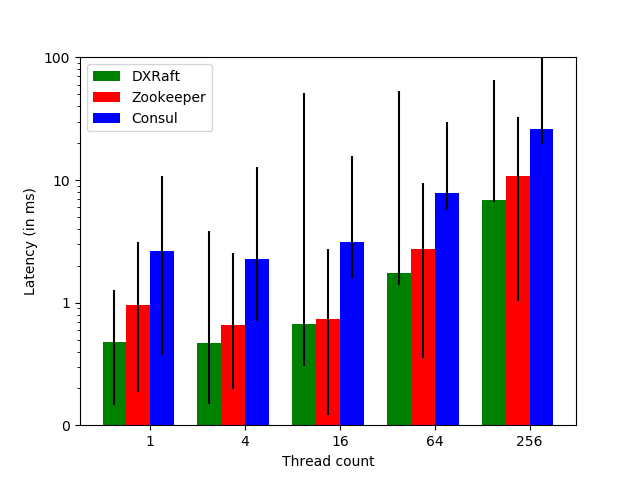
\includegraphics[width=\textwidth]{img/latency.png}
		\caption{100\% Writes.}
	\end{subfigure}
	\begin{subfigure}[t]{0.45\textwidth}
		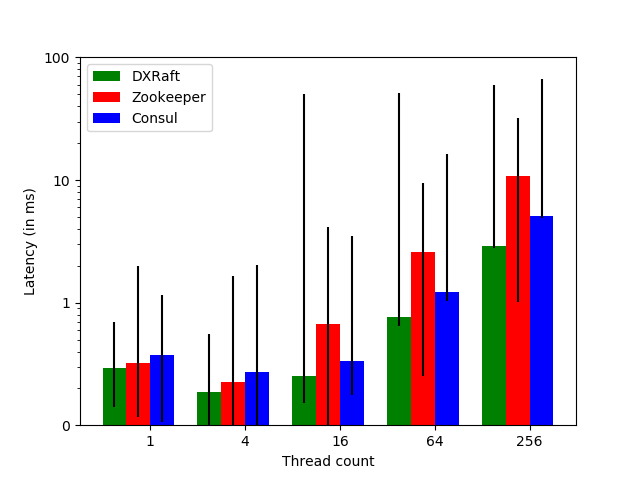
\includegraphics[width=\textwidth]{img/latency2.png}
		\caption{25\% Writes, 75\% Reads.}
	\end{subfigure}
	\caption{Latenzen der Systeme. Der Benchmark wurde mit einem Client und drei Server durchgeführt.}
	\label{fig:latency}
\end{figure}

\section{Durchsatz}

\begin{figure}[t]
	\centering
	\begin{subfigure}[t]{0.45\textwidth}
		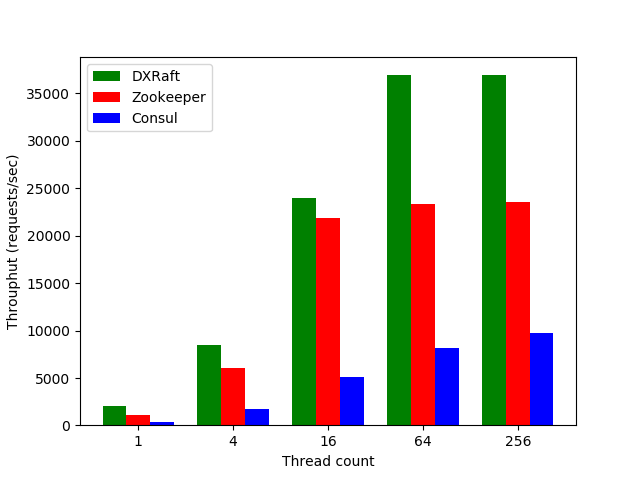
\includegraphics[width=\textwidth]{img/throughput.png}
		\caption{100\% Writes.}
	\end{subfigure}
	\begin{subfigure}[t]{0.45\textwidth}
		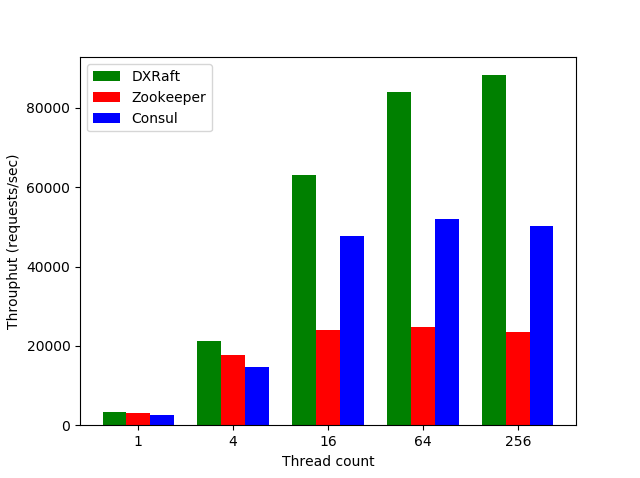
\includegraphics[width=\textwidth]{img/throughput2.png}
		\caption{25\% Writes, 75\% Reads.}
	\end{subfigure}
	\caption{Durchsatz der Systeme. Der Benchmark wurde mit einem Client und drei Server durchgeführt.}
	\label{fig:througput}
\end{figure}


\section{Latenz in DXRaft}
\label{dxraft-latency}

\begin{figure}[t]
	\centering
	\begin{subfigure}[t]{1\textwidth}
		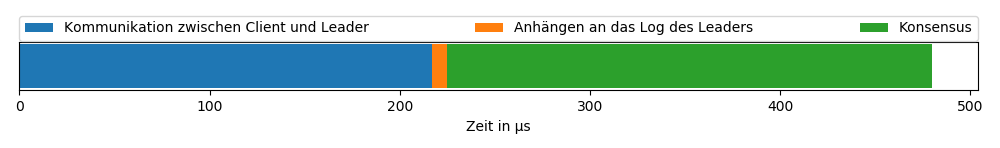
\includegraphics[width=\textwidth]{img/request_avg_timing.png}
		\caption{Durchschnittliche Anfrage.}
	\end{subfigure}
	\begin{subfigure}[t]{1\textwidth}
		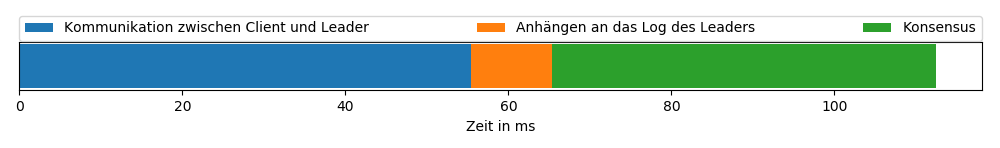
\includegraphics[width=\textwidth]{img/request_max_timing.png}
		\caption{Maximale Zeiten.}
	\end{subfigure}
	\begin{subfigure}[t]{1\textwidth}
		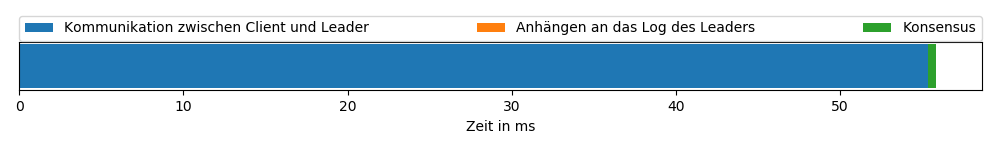
\includegraphics[width=\textwidth]{img/request_longest_timing.png}
		\caption{Längste Anfrage.}
	\end{subfigure}
\end{figure}

\section{Leader Election}

\begin{figure}[t]
	\centering
	\begin{subfigure}[t]{0.45\textwidth}
		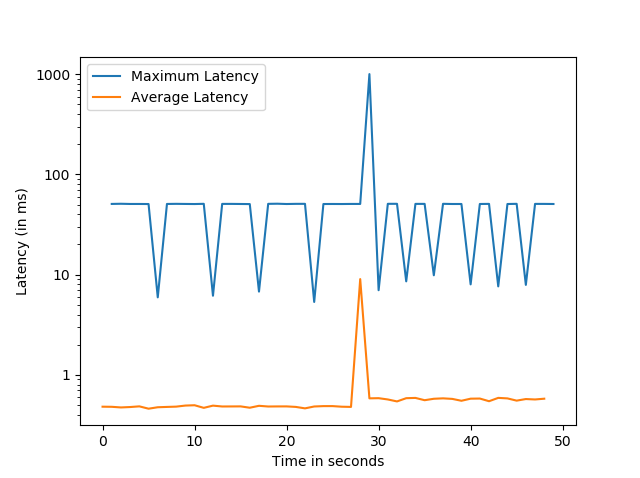
\includegraphics[width=\textwidth]{img/leader_crash_dxraft.png}
		\caption{DXRaft.}
	\end{subfigure}
	\begin{subfigure}[t]{0.45\textwidth}
		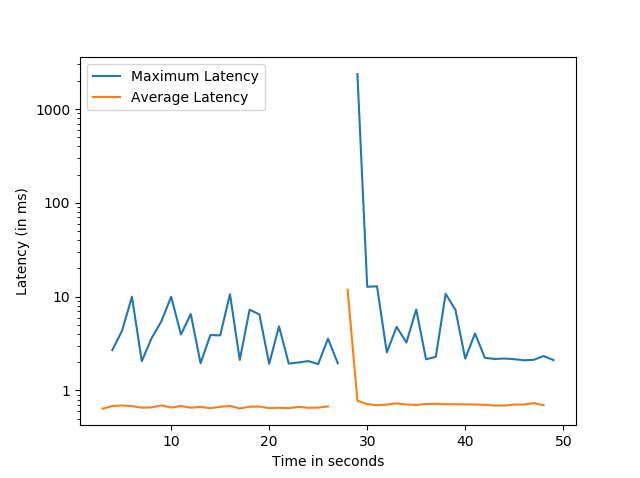
\includegraphics[width=\textwidth]{img/leader_crash_zk.png}
		\caption{Zookeeper.}
	\end{subfigure}
	\begin{subfigure}[t]{0.45\textwidth}
		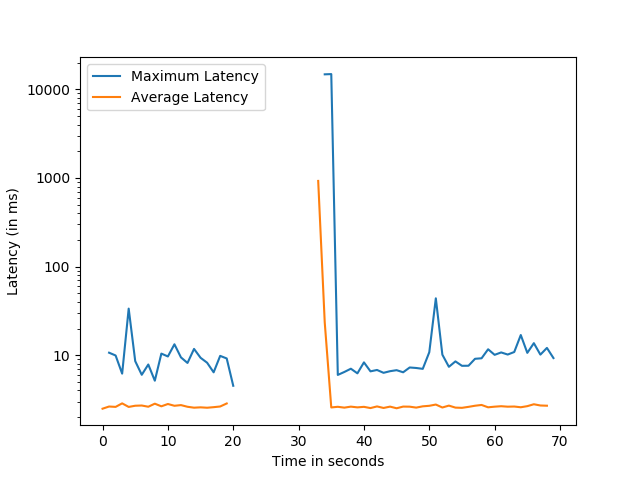
\includegraphics[width=\textwidth]{img/leader_crash_consul.png}
		\caption{Consul.}
	\end{subfigure}
	\caption{Latenz bei einem Leader-Crash.}
\end{figure}

